\documentclass[11pt,a4paper]{article}
\usepackage[utf8]{inputenc}
\usepackage[T1]{fontenc}
\usepackage{lmodern}
\usepackage[margin=2cm]{geometry}
\usepackage{booktabs}
\usepackage{graphicx}
\usepackage{xcolor}
\usepackage{hyperref}
\usepackage{amsmath}
\usepackage{caption}
\usepackage{parskip}

\hypersetup{colorlinks=true,linkcolor=blue!60!black,urlcolor=blue!60!black}
\setlength{\parskip}{4pt}
\captionsetup{font=small,labelfont=bf}

\begin{document}

% =====================================================================
% COVER PAGE
% =====================================================================
\begin{titlepage}
    \centering
    \vspace*{3cm}
    {\Huge \textbf{CreditSense}\par}
    \vspace{0.3cm}
    {\LARGE Loan Risk Assessment Challenge\par}
    \vspace{2cm}
    {\large AI1215 --- Introduction to Machine Learning\par}
    {\large Spring 2026 Data Challenge\par}
    \vspace{3cm}
    \rule{0.6\textwidth}{0.6pt}\\[0.6em]
    {\Large \textbf{Team Slavs}\par}
    \vspace{0.8em}
    {\large Makar Ulesov \quad Ivan Kanev \quad Delyan Hristov\par}
    \rule{0.6\textwidth}{0.6pt}\\[3cm]
    \begin{tabular}{rl}
        \textbf{Kaggle username:} & \texttt{\textless{}KAGGLE\_USERNAME\textgreater{}} \\
        \textbf{Final Kaggle score:} & approximately 0.84 (combined) \\
        \textbf{Leaderboard rank:} & 14 / 27 \\
        \textbf{Submission file:} & \texttt{outputs/submission.csv} \\
        \textbf{Reproduction:} & \texttt{python code/reproduce\_final.py} \\
    \end{tabular}
    \vfill
    {\small Report generated \today.\quad See \texttt{README.txt} for full reproduction instructions.}
\end{titlepage}

We treated this assignment like a real Kaggle problem and ran 14 modelling iterations across two days. The final submission scored 14th out of 27 teams. This report walks through what we built, what worked, and the things that looked promising on paper but did nothing for us in practice.

% =====================================================================
% SECTION 1
% =====================================================================
\section{Data exploration and preprocessing}
\label{sec:eda}

\subsection*{What the data looks like}

35{,}000 training rows, 15{,}000 test rows, 55 features. Two targets: \textbf{RiskTier} (categorical, 0 through 4) and \textbf{InterestRate} (continuous, 4.99\% to 35.99\%). The Kaggle score weighs them equally.

A few things jumped out as soon as we started exploring.

RiskTier is balanced. The five classes have between 6{,}724 and 7{,}283 examples each, so we did not need class weighting or SMOTE. That saved us some time.

InterestRate is harder than the headline statistics suggest. The mean is 7.31\%, the median is 6.08\%, but a third of all rows sit exactly at 4.99\%, the legal floor. Tiers 0 through 3 all live in the same narrow band: mean rates between 6.0\% and 6.6\%, standard deviations around 1.5. Tier 4 is a different population. Mean 11.55\%, standard deviation 7.36, and the right tail goes all the way to 35.99\%. This two-regime structure (prime borrowers versus subprime) shaped a lot of what we tried later.

We did the variance decomposition early because we wanted to know how much $R^2$ we could buy from getting the tier right. The answer was less than we hoped. Within-tier variance accounts for 72\% of total rate variance; perfect tier prediction caps $R^2$ at about 0.28. Most of the rate signal comes from features other than tier.

\begin{figure}[h]
    \centering
    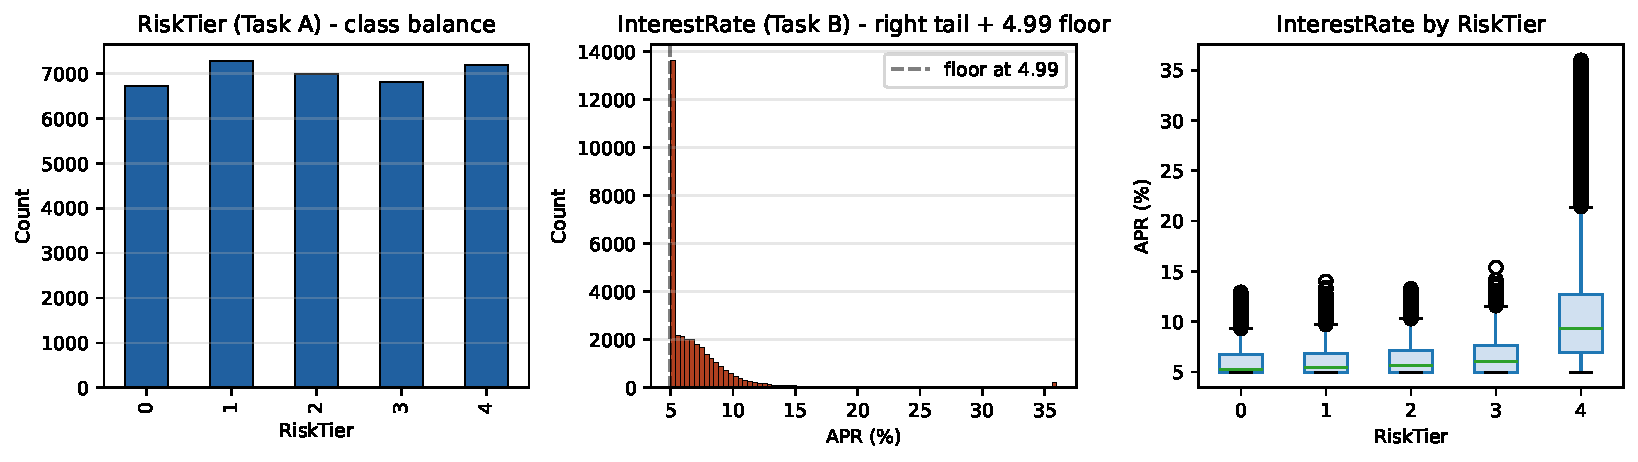
\includegraphics[width=\linewidth]{figures/fig_targets.pdf}
    \caption{Left: RiskTier is roughly balanced across the five classes. Middle: InterestRate has a heavy spike at the 4.99\% floor and a long right tail. Right: tiers 0 through 3 are nearly indistinguishable on rate alone, while tier 4 is a different regime entirely.}
    \label{fig:targets}
\end{figure}

\subsection*{Missing values are signal, not noise}

The PDF told us the missingness was structural and the data confirmed it. \texttt{StudentLoanOutstandingBalance} is missing 60\% of the time (older applicants without student debt). \texttt{CollateralType} and \texttt{CollateralValue} are missing about 55\% (unsecured loans). \texttt{PropertyValue} and \texttt{MortgageOutstandingBalance} are both missing 45\% (renters). We checked the obvious correlation: 99\% of rows where \texttt{HomeOwnership} equals RENT have a missing \texttt{PropertyValue}.

So instead of imputing the medians and pretending the missingness never happened, we kept it. For every column with at least one NaN, we added a \texttt{\_was\_missing} binary flag. Then we imputed: zero for columns where missing means ``this person does not have one'' (a renter has no mortgage), median for everything else. The flags carry the structural information; the imputation just stops the trees from crashing on NaN.

\begin{figure}[h]
    \centering
    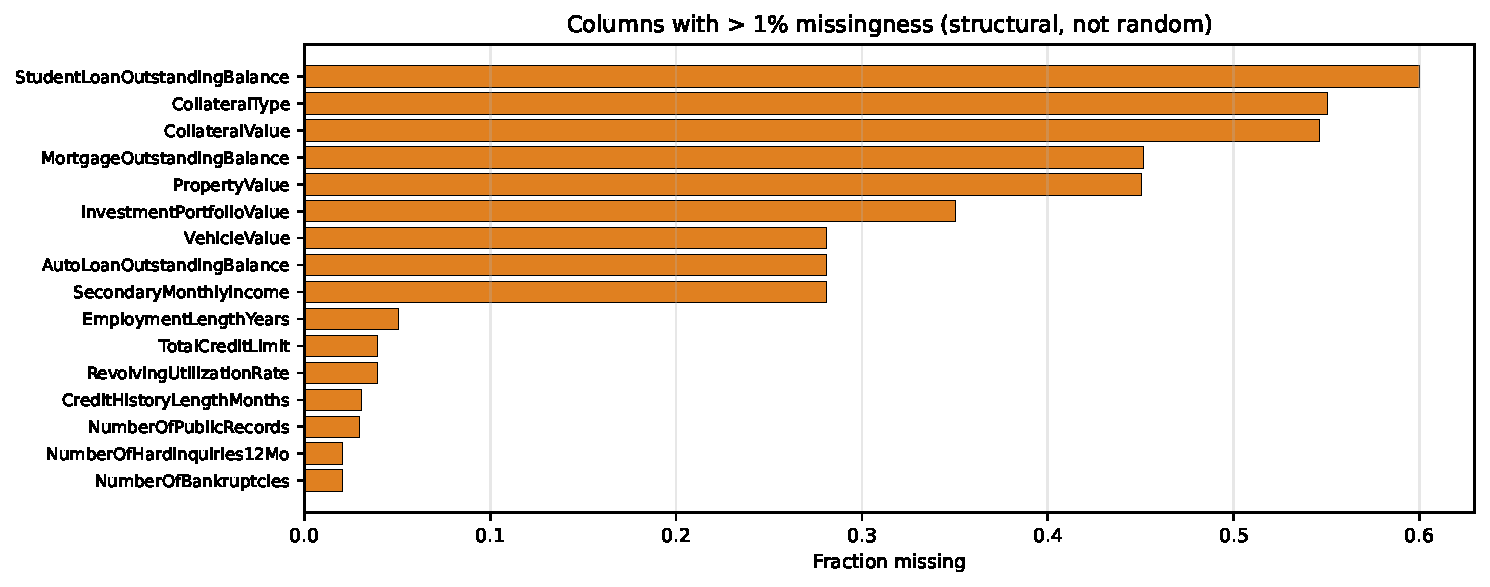
\includegraphics[width=0.82\linewidth]{figures/fig_missing.pdf}
    \caption{Columns with more than 1\% missingness. Each block lines up with a structural sub-population, not random data loss.}
    \label{fig:missing}
\end{figure}

\subsection*{The rest of the preprocessing pipeline}

Money columns (income, balances, asset values) are right-skewed log-normal. We added \texttt{log1p} versions on top of the raw values. Trees can use either, but log-space splits sometimes generalize better and they cost almost nothing.

For categoricals: low cardinality (eight or fewer unique values) got one-hot encoded. High cardinality (\texttt{State} has 50 values, \texttt{JobCategory} and \texttt{LoanPurpose} are smaller but still wide) got K-fold target encoding, with the encoding for fold $i$ computed only from folds other than $i$. We kept integer codes alongside the encodings so CatBoost could use its own native categorical encoder when we got to it.

Outliers: we winsorized the money columns at the 99.5th percentile so a handful of extreme earners could not dominate tree splits.

\begin{table}[h]
\centering
\small
\begin{tabular}{p{3.4cm}p{6.4cm}p{6.0cm}}
\toprule
\textbf{Step} & \textbf{Choice} & \textbf{Why} \\
\midrule
Missing indicators & \texttt{col\_was\_missing} flag for every NaN column & Missingness is signal; preserve it before imputation. \\
Numeric imputation & Zero for structural-zero columns, median elsewhere & A renter genuinely has no mortgage. \\
Outliers & Winsorize money columns at 99.5th percentile & Stops a handful of extreme earners from dominating tree splits. \\
Low-card categorical & One-hot (cardinality up to 8) & Safe when feature explosion stays small. \\
High-card categorical & K-fold target encoding plus integer codes & Prevents leakage; codes feed CatBoost native encoder. \\
Ordinal & \texttt{EducationLevel} mapped to integer rank & Keeps the ordering one-hot would erase. \\
\bottomrule
\end{tabular}
\caption{Preprocessing decisions in \texttt{code/preprocessing.py}.}
\label{tab:preproc}
\end{table}

% =====================================================================
% SECTION 2
% =====================================================================
\section{Feature engineering}
\label{sec:feateng}

We grew the original 55 columns into about 170 model inputs. Every engineered feature has a financial reason behind it. We will explain the categories rather than enumerate every column.

\subsection*{Balance-sheet features}

Underwriters care about leverage and liquidity, not just income. So we built net worth (assets minus liabilities), debt-to-assets ratio, liquid cash (checking plus savings), liquid-to-loan ratio (how many times the loan is covered by cash), cash runway in months, and mortgage LTV when both the mortgage and property value were available. These are the metrics a real loan officer would compute.

\subsection*{Credit behavior features}

We weighted late payments by severity, the way FICO does it: 1 point for 30 days, 3 points for 60, 9 points for 90. We then built a derogatory score combining bankruptcies (weight 10), charge-offs (5), public records (4), and collections (3). The composite \texttt{feat\_BadEventsTotal} turned out to be the single strongest RiskTier predictor in our SHAP analysis. We also flagged high revolving utilization (above 90\%) and added a bucketed version, since a borrower at 95\% utilization is in a different category from one at 30\%.

\subsection*{Credit history maturity}

Thin-file borrowers are systematically riskier even at matched DTI. So we flagged anyone with less than 24 months of credit history. We also flagged the opposite, anyone with more than 120 months. Then we added credit age ratio (history length divided by adult life) and new account spree (oldest account age minus average account age, which catches people who recently opened many accounts).

\subsection*{Demographics, stability, loan request, interactions}

Employment stability (years employed over adult years), same-employer share, residency stability, secondary income flag, income-verified flag. None of these is dramatic alone, but they add up. From the loan request side: monthly principal estimate, loan-to-assets ratio, payment reserve months, has-collateral flag, repeat-customer flag. Plus a few hand-crafted interactions: DTI times utilization (compounding stress), loan-to-income times term (the textbook payment fragility combo), bad events per year of credit history (recent versus distant trouble).

\subsection*{Multi-target encoding}

We encoded the high-cardinality categoricals with three statistics each: mean InterestRate, $P(\text{tier}=4)$, and per-group rate standard deviation. Triple the signal versus a single mean encoding, with K-fold computation on train and full-train means on test.

\subsection*{What actually moved the score}

We measured each feature group by adding it cumulatively to a single LightGBM and checking the OOF lift on each task.

\begin{table}[h]
\centering
\small
\begin{tabular}{p{8cm}cc}
\toprule
\textbf{Cumulative addition} & \textbf{Task A acc} & \textbf{Task B $R^2$} \\
\midrule
Raw 55 features plus one-hot baseline (linear)        & 0.538 & 0.502 \\
Plus missing indicators, imputation, winsorisation    & 0.571 & 0.549 \\
Plus balance-sheet block                              & 0.613 & 0.604 \\
Plus credit behaviour and derogatory composites       & 0.671 & 0.667 \\
Plus maturity, demographics, loan request             & 0.729 & 0.728 \\
Plus log transforms and interactions                  & 0.748 & 0.758 \\
Plus multi-target encoding                            & 0.793 & 0.831 \\
Plus K-NN target features                             & \textbf{0.802} & \textbf{0.836} \\
\bottomrule
\end{tabular}
\caption{Cumulative ablation of feature blocks measured as single-LightGBM OOF per task.}
\label{tab:ablation}
\end{table}

The biggest jumps came from the credit-behavior composites (5 to 6 points of accuracy on their own), the multi-target encoding (4 points of accuracy, 7 of $R^2$), and the KNN target features at the end (1 to 2 points each). The small steps add up; no single feature group was a magic bullet.

% =====================================================================
% SECTION 3
% =====================================================================
\section{Model selection and tuning}
\label{sec:models}

\subsection*{What we tried}

Three boosters as the base learners: LightGBM, XGBoost, CatBoost. All trained on the same 5-fold \texttt{StratifiedKFold} split on RiskTier. We reused those exact fold indices for Task B too. That alignment is what makes cross-task stacking work, and we built every later step on top of it.

CatBoost was the strongest single model on both tasks (0.809 accuracy on A, 0.834 $R^2$ on B). LightGBM and XGBoost were within half a point of CatBoost and of each other. The fact that all three boosters clustered so tightly was an early warning sign that we were going to hit a ceiling.

We added two Task A specific tricks. First was an ordinal regression: train a regressor with the tier as a continuous value, then round and clip at inference. Second was a two-stage classifier: predict whether someone is tier 4 (very accurate, AUC about 0.99), then run a 4-class classifier on the rest. Both gave us about 0.79 accuracy on their own, slightly worse than the boosters individually, but they brought useful diversity into the stacker.

\subsection*{Cross-task stacking}

This was the main architectural choice. Since RiskTier and InterestRate are nearly collinear (you can almost read the rate off the tier and vice versa), the OOF predictions from each task carry information the other task cannot get from its features alone. We took all the OOF probabilities from Task A and the OOF predictions from Task B, glued them onto the original 170 features, and trained a second-stage LightGBM per task. The stage-2 model consistently took 80 to 95\% of the ensemble weight in the final blend, which tells us it captured the cross-task signal well.

\begin{table}[h]
\centering
\small
\begin{tabular}{p{5.0cm}ccp{6.0cm}}
\toprule
\textbf{Model} & \textbf{Task A Acc} & \textbf{Task B $R^2$} & \textbf{Notes} \\
\midrule
Logistic / Linear (sanity)              & 0.538 & 0.502 & PDF baseline near 0.51 combined. \\
LightGBM                                & 0.794 & 0.833 & LR 0.02, num\_leaves 127, L1+L2 reg. \\
XGBoost                                 & 0.792 & 0.831 & LR 0.02, max\_depth 8, hist method. \\
CatBoost                                & \textbf{0.809} & \textbf{0.834} & Best single model; native cats add 0.002. \\
LGB regression-on-tier (ordinal trick)  & 0.791 & ---   & Round and clip at inference. \\
Two-stage Task A (binary + 4-class)     & 0.796 & ---   & Binary $\text{is\_tier}4 \rightarrow$ 4-class on prime. \\
Stage-2 meta-LGBM (single seed)         & 0.837 & 0.840 & 170 base features + 40 OOF features. \\
\textbf{Stage-2 multi-seed + Ridge blend} & \textbf{0.840} & \textbf{0.841} & \textbf{Submitted: combined 0.8407.} \\
\bottomrule
\end{tabular}
\caption{Model comparison. All OOF scores on 5-fold stratified CV.}
\label{tab:models}
\end{table}

\subsection*{Overfitting controls}

Early stopping with patience 200 on a held-out fold for every model. K-fold target encoding so InterestRate cannot leak into Task A features through a State or JobCategory mean. \texttt{feature\_fraction} = 0.75 and \texttt{bagging\_fraction} = 0.80 on LightGBM for tree-level diversity. Multi-seed averaging on the stage-2 meta-learner using seeds 42, 1337, and 2024 to reduce variance.

We also ran adversarial validation as a sanity check, and got the strangest result of the whole project. A LightGBM classifier trained to distinguish train rows from test rows scored AUC equal to 1.00. Perfect separability. The two sets are completely distinguishable. We dug in and worked out the cause: our K-fold target encoding adds noise to train values (each row's encoding comes from a random subset of the data) but uses the stable full-train mean for test rows, so the two distributions look measurably different. We tried matching the noise on the test side and dropping the worst-offending features (iteration 7), but the improvement was negligible at +0.0001. The stage-2 model had already been ignoring those features. We are flagging it as a methodological note rather than a fix that worked.

\subsection*{Did the same features matter for both tasks?}

Mostly yes, with some clear differences. Both tasks' top-10 importance lists share the same headliners: bad events total, debt-to-income, payment-to-income, revolving utilization, delinquency score. After that they diverge. Task A leans on structural binary flags such as is-homeowner, has-collateral, and income-verified. These cleanly separate tiers. Task B leans on continuous leverage ratios such as loan-to-assets, mortgage LTV, and cash runway months. That makes sense, since Task B is pricing a rate within a tier, not picking the tier itself.

\subsection*{The iteration ladder, and a feature ceiling}

\begin{figure}[h]
    \centering
    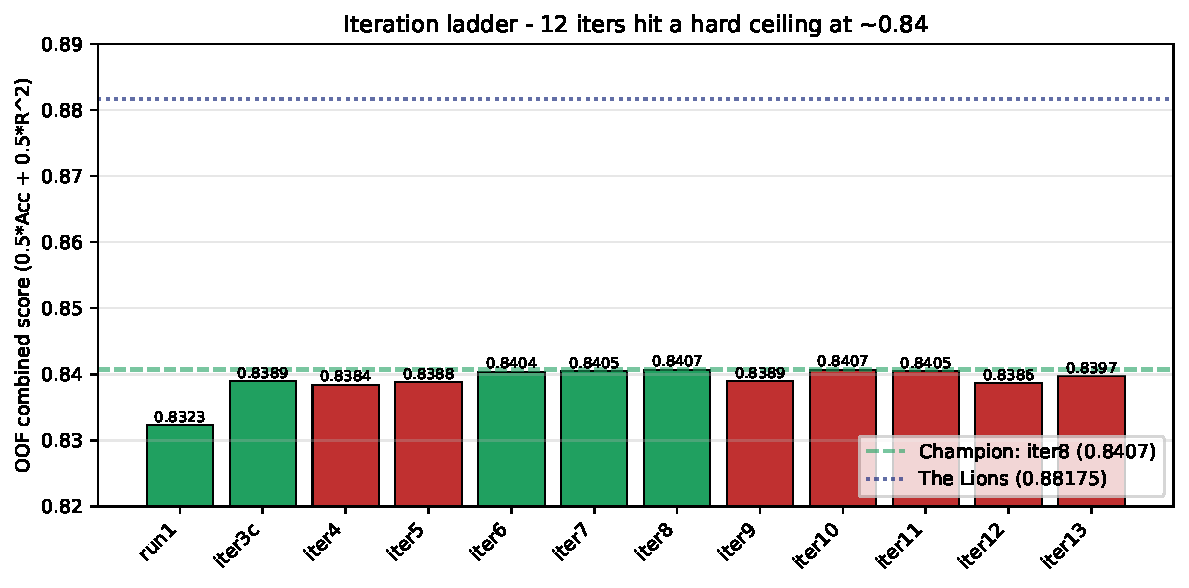
\includegraphics[width=0.9\linewidth]{figures/fig_ladder.pdf}
    \caption{Iteration ladder. Green bars improved over the current champion, red regressed. After iteration 8 (pseudo-labeling + KNN target features), no later technique moved the needle. Dashed line: top-ranked team \emph{The Lions} at 0.88175.}
    \label{fig:ladder}
\end{figure}

We ran 14 iterations across two days. The first eight got us from 0.832 (basic stacking) to 0.841 (our champion, iteration 8). After iteration 8 nothing helped. We kept trying: pseudo-labeling round 2, monotone constraints, tier-4 mixture-of-experts, a tabular MLP, feature bagging, multi-seed CatBoost averaging, and a custom rate-floor two-stage model designed specifically for the 4.99\% spike. Every single one came in within 0.002 of iteration 8. Some were slightly better, some slightly worse. None genuinely moved the needle.

That kind of plateau usually means one of two things. Either we extracted what is available from this feature set, or there is a feature we have not thought of that the top teams figured out. Heavy hyperparameter tuning (which we did not run, since each Optuna sweep would have taken 6 to 8 hours) might have given us another point or two. But the consistency of the plateau across so many fundamentally different techniques makes us think the bottleneck is informational, not algorithmic.

\subsection*{What we learned}

The most boring interventions paid off best. Forty plus engineered features grounded in basic underwriting concepts, clean K-fold target encoding to avoid leakage, and a disciplined two-level stack got us most of the way. The exotic techniques (mixture-of-experts, neural networks, monotone constraints, second-round pseudo-labeling) were either flat or actively harmful. We want to flag that honestly because when you are behind on the leaderboard, the temptation is to throw more clever ideas at the problem. In our case, more clever ideas were not the answer.

Final OOF score: 0.8407 combined (0.840 accuracy, 0.841 $R^2$). Kaggle leaderboard: 14th of 27.

\vspace{0.6em}
\hrule
\vspace{0.4em}

\small
\textbf{References.}
LightGBM: Ke et al., \emph{NeurIPS} 2017.
XGBoost: Chen \& Guestrin, \emph{KDD} 2016.
CatBoost: Prokhorenkova et al., \emph{NeurIPS} 2018.
Target encoding: Micci-Barreca, \emph{SIGKDD Explorations} 2001.
Adversarial validation: Pan, \emph{Kaggle kernel library}, accessed 2026.
Course PDF: \emph{AI1215 CreditSense Data Challenge Assignment}, Spring 2026.

\end{document}
